\chapter{Suporte}

\section{Introdução}
O suporte da Eurotux está disponível através de uma ferramenta criada para facilitar a consulta e estado dos pedidos. Esta ferramenta está acessível através da Web, e permite obter respostas a pedidos de informações e de help-desk de forma eficiente.

Sublinhamos que a utilização desta ferramenta é absolutamente essencial para garantir uma resposta rápida e o melhor acompanhamento dos problemas reportados à Eurotux. O recurso à ajuda telefónica poderá acontecer sempre que for essencial através do número +351 253 680 301. Para os clientes que tiverem o serviço de suporte disponível em horário não laboral será fornecido um numero de um telefone móvel.

\mbox{A ferramenta Web está acessível através do endereço \url{https://suporte.eurotux.com} (figura \ref{fig:rt1}).}

\begin{figure}[H]
\begin{center}
%\includegraphics[scale=0.45]{include/rt1}
\includegraphics[width=16cm,height=10.5cm]{include/img/rt1}
\end{center}
\caption{Página de Autenticação}
\label{fig:rt1}
\end{figure}

No ecrã que aparece imediatamente após o \emph{login}, existe uma coluna no lado direito identificada como \emph{Quick Search} em que existe um único item (\emph{queue}).
É nessa \emph{queue} que estarão os pedidos de suporte/help-desk (\emph{tickets}) ainda abertos
(open) (figura \ref{fig:rt2}).

\begin{figure}[H]
\begin{center}
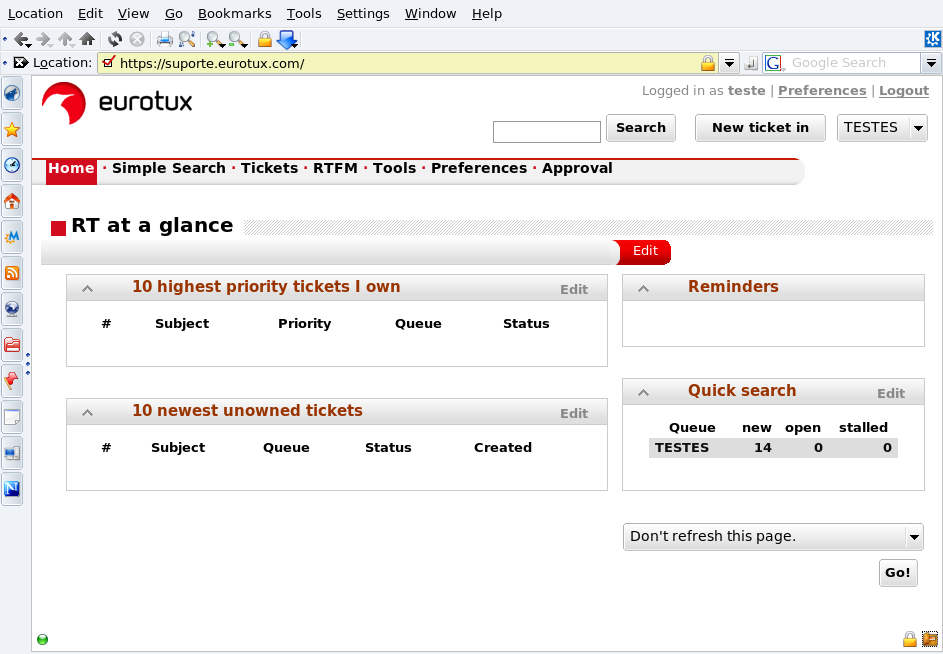
\includegraphics[width=16cm]{include/img/rt2}
\end{center}
\caption{Página Inicial}
\label{fig:rt2}
\end{figure}

\section{Criar \emph{Ticket}}
Para criar um \emph{ticket} será necessário seleccionar \emph{New Ticket In} e, pelo menos, preencher o campo \emph{Subject} e descrever o pedido em \emph{Describe the issue below} (ver figura \ref{fig:rt3}). Desta forma o pedido/problema fica registado e acessível aos técnicos da Eurotux que irão aceder a informação que foi registada e à qual darão o seguimento adequado.

A \emph{comunidade de utilizadores} que acede a uma \emph{queue} recebe sempre por email o conteúdo que for colocado nessa \emph{queue} por qualquer um dos membros da \emph{comunidade de utilizadores}. A \emph{comunidade de utilizadores} é normalmente constituída pelos endereços do cliente dessa \emph{queue} (um ou mais) e pelos endereços dos técnicos da Eurotux.

Após a recepção do email mencionado no parágrafo anterior é possível responder a essa mensagem fazendo um \emph{reply} normal, escrevendo no corpo da mensagem as informações que se pretende transmitir e de imediato essa informação será adicionada ao \emph{ticket} em causa ficando imediatamente também acessível via Web (sem necessidade de aceder directamente à ferramenta). \textbf{NOTA}: A aplicação web só registará mensagens cujo o endereço de email coincida com um dos emails registados na \emph{comunidade de utilizadores}, o que significa se for usado qualquer outro, a mensagem não ficará registada.

Quando for efectuado reply às mensagens deve-se retirar o máximo de informação não relevante da mensagem e colocar só o que corresponde a informação nova porque a ferramenta por si já constitui um histórico das diversas interacções.


\begin{figure}[H]
\begin{center}
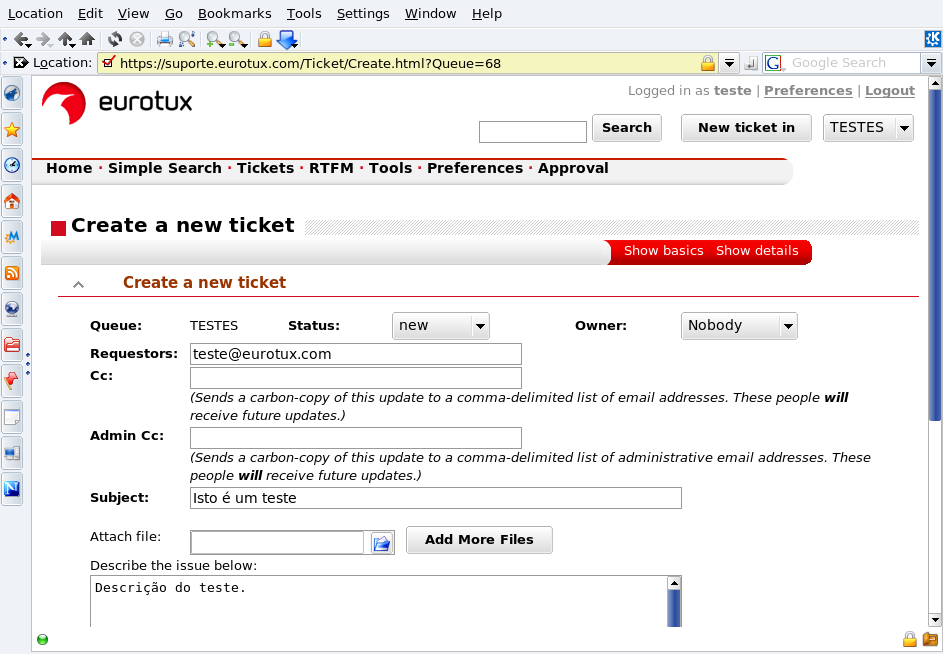
\includegraphics[width=16cm]{include/img/rt3}
\end{center}
\caption{Criação de um \emph{Ticket}}
\label{fig:rt3}
\end{figure}

\section{Fecho de \emph{Tickets}}
Os \emph{tickets} devem ser encerrados pelo próprio cliente, constituindo o seu encerramento uma forma de aprovação e validação das actividades desenvolvidas, significando ainda que a intervenção está concluída. Para encerrar o \emph{ticket} basta seleccionar a opção \emph{Resolve} que aparece um pouco abaixo do canto superior direito do ecrã onde se está a visualizar um determinado \emph{ticket}.

Os \emph{tickets} depois de encerrados não aparecerão na visualização por omissão.

\section{Pesquisas de \emph{Tickets}}
Podem ser efectuadas pesquisas nos \emph{tickets} encerrados e ainda abertos, seleccionando no menu localizado na parte superior da página, o link \emph{Tickets}, aparecendo um menu denominado \emph{Query Builder} (ver figura \ref{fig:rt4}). De seguida deverão ser preenchidos os campos adequados para obter os \emph{tickets} que obedeçam aos critérios definidos.

Sabendo o número do \emph{ticket} é possível visualizá-lo imediatamente bastando para isso introduzir esse número na caixa que diz \emph{Search} (do lado direito, quase no topo do ecrã).

\begin{figure}[H]
\begin{center}
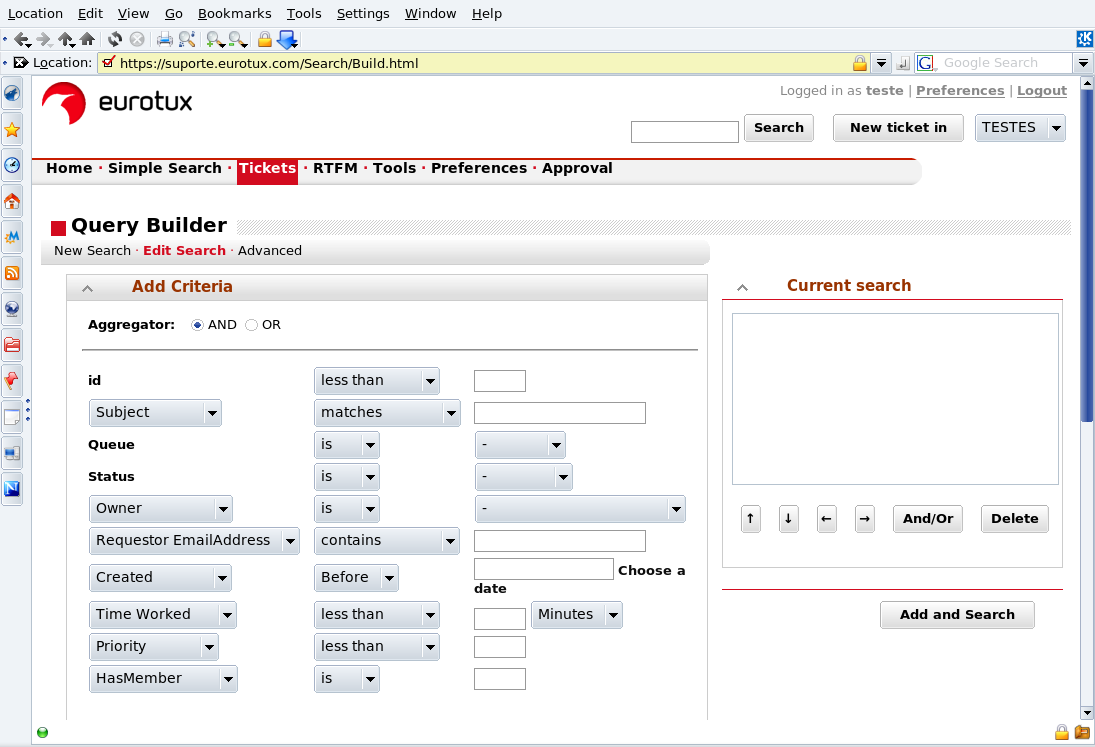
\includegraphics[width=16cm,height=10.5cm]{include/img/rt4}
\end{center}
\caption{Procurar \emph{Tickets}}
\label{fig:rt4}
\end{figure}

\section{Preferências}
No menu do lado esquerdo aparece uma opção denominada \emph{Preferences} (ver figura \ref{fig:boot}) onde pode ser alterada a password de acesso à ferramenta web (\underline{é conveniente fazê-lo}), alterar o idioma (aconselhamos que optem pelo inglês), etc.

\begin{figure}[H]
\begin{center}
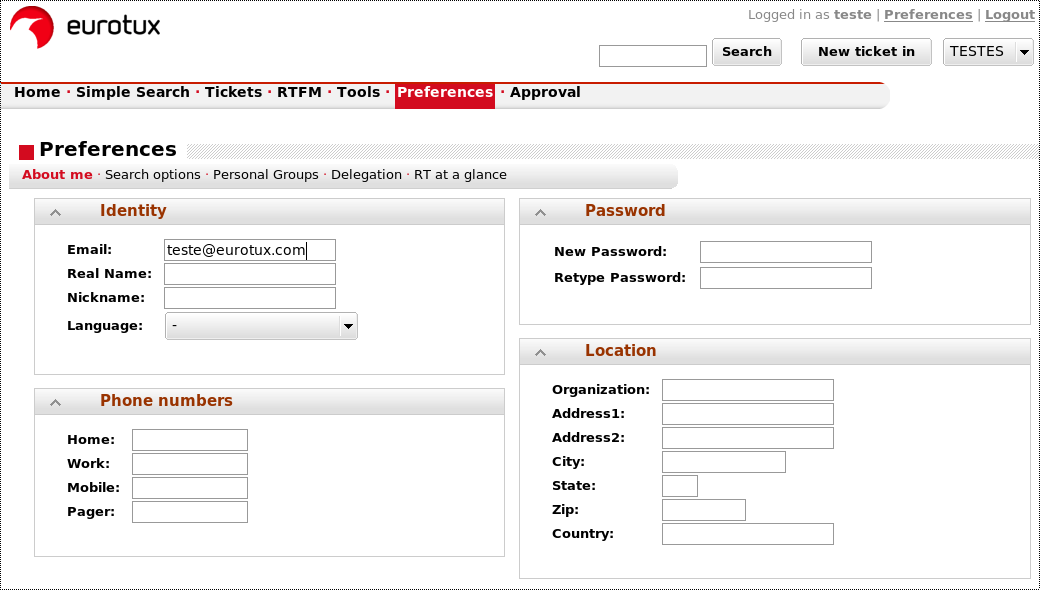
\includegraphics[width=16cm,height=12cm]{include/img/rt5}
\end{center}
\caption{Alterar Preferências}
\label{fig:boot}
\end{figure}


\section{Observações}
Qualquer dúvida ou informações adicionais relativamente à utilização desta ferramenta podem ser obtidas através do \emph{email} \texttt{tec@eurotux.com}.

Seria importante que, logo que possível, fossem efectuados alguns testes de utilização à ferramenta. Sugerimos a criação de \emph{ticket} com o \emph{Subject} ''teste`` para experimentar todas as opções mencionadas. Se assim acontecer será possível concretizar uma aprendizagem progressiva no uso da ferramenta.
